% =====================================================================
%  Prabhavit Gupta - Tailored CV for BASF
%  Role:     AI Engineer - Agentic Coding (m/f/d)
%  Location: Madrid, Spain (Hybrid)
%  Compile:  tectonic cv/main_BASF_AIEngineer.tex OR lualatex / pdflatex
%  Needs:    photo.jpg in cv/
%  Rules:    ONE PAGE. 0 em-dashes. Plain voice. Clickable links.
% =====================================================================
\documentclass[a4paper,10pt]{article}

\usepackage[T1]{fontenc}
\usepackage[utf8]{inputenc}
\usepackage[top=0.7cm,bottom=0.7cm,left=1.0cm,right=1.0cm]{geometry}
\usepackage{titlesec}
\usepackage{enumitem}
\usepackage{hyperref}
\usepackage{xcolor}
\usepackage{graphicx}

\definecolor{accent}{HTML}{1F4E78}
\hypersetup{colorlinks=true, urlcolor=accent, linkcolor=accent}
\pagestyle{empty}
\setlength{\parindent}{0pt}

\titleformat{\section}{\large\bfseries\color{accent}}{}{0em}{}[\vspace{-0.6em}\rule{\textwidth}{0.8pt}]
\titlespacing{\section}{0pt}{2pt}{1pt}

\newcommand{\role}[4]{%
 \textbf{#1} \hfill \textbf{#2}\\[1pt]%
 \textit{#3} \hfill \textit{#4}\\[2pt]%
}
\setlist[itemize]{leftmargin=1.2em, itemsep=0pt, topsep=1pt, parsep=0pt}

\begin{document}

% ================= HEADER =================
\begin{minipage}[c]{0.80\textwidth}
 {\Huge\bfseries Prabhavit Gupta}\\[3pt]
 {\color{accent}\large AI Engineer: Agentic Coding, Developer Experience \& Core Systems}\\[5pt]
 {\footnotesize +39 351 610 7807 ~$\vert$~
 \href{mailto:prabhavitg@gmail.com}{prabhavitg@gmail.com} ~$\vert$~
 \href{https://www.linkedin.com/in/prabhavit/}{linkedin.com/in/prabhavit} ~$\vert$~
 \href{https://github.com/prab-gupta}{github.com/prab-gupta} ~$\vert$~
 Venice, Italy}
\end{minipage}\hfill
\begin{minipage}[c]{0.18\textwidth}
 \raggedleft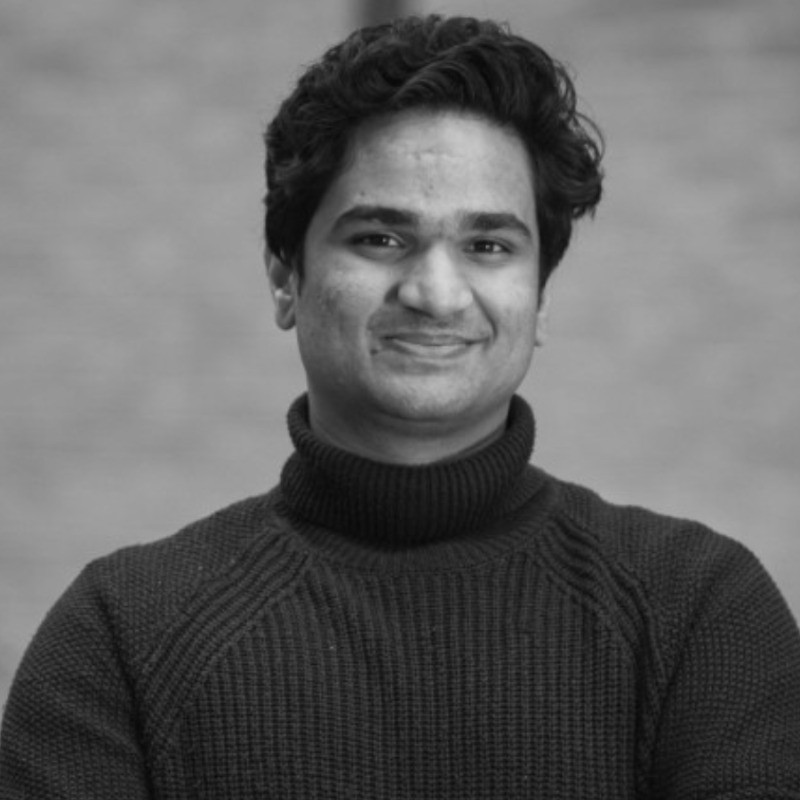
\includegraphics[width=2.0cm]{photo.jpg}
\end{minipage}
\vspace{-2pt}

% ================= SUMMARY =================
\section{Summary}
Software engineer specializing in agentic coding workflows, developer enablement, and production LLM orchestration. Daily hands-on practitioner with Claude Code, Cursor, and GitHub Copilot, leveraging tool-calling mechanisms, Model Context Protocol (MCP), and automated test harnesses to accelerate engineering velocity and refactor legacy architectures. Proven track record migrating live production platforms, architecting reliable data extraction pipelines with human-in-the-loop review, and evaluating models on real-world engineering tasks. Core technical depth in TypeScript, Python, Node.js, and CI/CD reliability.

% ================= SKILLS =================
\section{Skills}
\begin{itemize}
 \item \textbf{Agentic Coding \& AI Tooling:} Claude Code, Cursor, GitHub Copilot, Codex, Model Context Protocol (MCP), LLM APIs (Anthropic Claude, OpenAI), tool calling, context window management, prompt engineering, agent evaluation and benchmarking
 \item \textbf{Software Engineering \& Architecture:} TypeScript, Python, JavaScript, Node.js, Next.js, FastAPI, Laravel (PHP), REST APIs, OpenAPI specs, Docker, CI/CD, Git/GitHub, Linux
 \item \textbf{Refactoring \& DevEx Enablement:} Legacy stack migration, test harness engineering, developer experience (DevEx), golden paths, automated test suites (Playwright, Postman, Jest), system refactoring, failure recovery
 \item \textbf{Data Platforms \& Integrations:} PostgreSQL, Supabase, Redis, vector embeddings, RAG architectures, n8n, webhooks, third-party API integrations (CRM, booking platforms, cloud services)
\end{itemize}

% ================= EXPERIENCE =================
\section{Experience}

\role{\href{https://flowspace.co}{FlowSpace.co}}{Mar 2024 - Aug 2026}{Lead Developer \& AI Engineer (Full-time, Freelance)}{London, UK (remote)}
\begin{itemize}
 \item Migrated a live marketplace off a legacy stack to coded Next.js and Laravel, scaling active users from 2,000 to 4,500+ without downtime.
 \item Integrated agentic workflows and Claude Code into daily engineering cycles, establishing automated test harnesses and prompt scaffolding that cut feature delivery cycles.
 \item Engineered an AI document ingestion pipeline (TypeScript, Claude API, n8n) extracting structured data from PDFs, spreadsheets, and web sources with human-in-the-loop review; 900+ listings processed.
 \item Deployed support agents operating over live platform data, implementing confidence scoring thresholds and deterministic fallback paths for edge cases.
\end{itemize}

\role{\href{https://get2germany.com}{Get2Germany.com}}{Jan 2024 - May 2024}{Developer \& Automation Specialist (Part-time)}{Berlin, Germany}
Built AI tools in n8n to aggregate, categorize, and serve courses and job listings, optimizing backend ETL pipelines and Google API integrations.\\[1pt]

\role{\href{https://clubee.com}{Clubee.com}}{Sep 2023 - Aug 2024}{Developer \& QA (Full-time, Freelance)}{Foetz, Luxembourg}
Integrated Clubee REST APIs across frontend modules, established automated unit test suites, and executed QA protocols for federation dashboards.\\[1pt]

\role{\href{https://tractionboard.co}{Tractionboard.co}}{Aug 2023 - Oct 2023}{Developer (Internship)}{Utrecht, Netherlands}
Integrated OpenAI/ChatGPT and Sendgrid APIs, built responsive frontend interfaces, and debugged core platform features.

% ================= PROJECTS =================
\section{Selected Projects \& Open Source}
\begin{itemize}
 \item \textbf{\href{https://github.com/prab-gupta/llm-doc-parser}{llm-doc-parser}} (Open Source): Built and published an end-to-end pipeline extracting structured JSON from raw documents using LLM tool calling, schema validation, and fallback mechanisms.
 \item \textbf{\href{https://smarturlink.com/}{Urlink}} (2025), Project Manager \& AI-Assisted Developer: Managed client requirements and built platform architecture using AI-assisted development tools (Claude Code, Next.js, Supabase), accelerating delivery timelines.
 \item \textbf{\href{https://ultrastrategy.com}{UltraStrategy}} (2024 - 2025), AI Automation Developer: Built an automated CV-parsing engine using LLM data extraction pipelines (n8n, Eden AI) across diverse candidate document profiles.
\end{itemize}

% ================= CERTIFICATIONS =================
\section{Certifications}
Microsoft Copilot Studio Agent Academy \textbullet\ Microsoft: Introduction to building AI agents \textbullet\ Microsoft Power Automate \textbullet\ Tray.AI Build Practitioner (Sep 2024)

% ================= EDUCATION =================
\section{Education}
\textbf{Ca' Foscari University of Venice} \hfill Oct 2020 - Jun 2024\\
BA Philosophy, International Studies \& Economics (Minor: Entrepreneurship)

% ================= AUTH =================
\vspace{2pt}
{\small \textbf{Work authorization:} Italian EU Long Term Residence Permit (unrestricted EU work rights, no visa sponsorship needed in Spain); available immediately. \quad \textbf{Languages:} English (fluent C2), Hindi (native), Italian (conversational).}

\end{document}